\documentclass[a4paper,12pt]{article} % добавить leqno в [] для нумерации слева
\usepackage[a4paper,top=1.3cm,bottom=2cm,left=1.5cm,right=1.5cm,marginparwidth=0.75cm]{geometry}
%%% Работа с русским языком
\usepackage{cmap}					% поиск в PDF
\usepackage[warn]{mathtext} 		% русские буквы в фомулах
\usepackage[T2A]{fontenc}			% кодировка
\usepackage[utf8]{inputenc}			% кодировка исходного текста
\usepackage[english,russian]{babel}	% локализация и переносы
\usepackage{physics}
\usepackage{multirow}
\usepackage{float}
\restylefloat{table}
\usepackage{graphicx}
\usepackage{wrapfig}
\usepackage{tabularx}
\usepackage{hyperref}
\usepackage[rgb]{xcolor}
\hypersetup{
colorlinks=true,urlcolor=blue
}

%%% Дополнительная работа с математикой
\usepackage{amsmath,amsfonts,amssymb,amsthm,mathtools} % AMS
\usepackage{icomma} % "Умная" запятая: $0,2$ --- число, $0, 2$ --- перечисление

%% Номера формул
\mathtoolsset{showonlyrefs=true} % Показывать номера только у тех формул, на которые есть \eqref{} в тексте.

%% Шрифты
\usepackage{euscript}	 % Шрифт Евклид
\usepackage{mathrsfs} % Красивый матшрифт

%% Свои команды
\DeclareMathOperator{\sgn}{\mathop{sgn}}

%% Перенос знаков в формулах (по Львовскому)
\newcommand*{\hm}[1]{#1\nobreak\discretionary{}
{\hbox{$\mathsurround=0pt #1$}}{}}

\begin{document}

	\begin{titlepage}
		\begin{center}
			\large Московский физико-технический институт\\
			(национальный исследовательский университет)\\
			\vspace{9cm}
			\large{Лабораторная работа №3}\\ \Huge{<<Свет, цвет и альбедо>>}
		\end{center}
		
		\vspace{10cm}
		{\par \raggedleft \large Выполнили:\\ Макаренко Николай\\ Тихомиров Андрей\\ Янаков Филипп\\ Б03-202\\}
	\end{titlepage}\
 
\section{Введение}
 
    \subsection{Цели}
При помощи компьютера, КМОП-матрицы, объектива и дифракционной решётки изучить зависимость альбедо отражающей поверхности от её цвета в видимой области спектра.
    \subsection{Задачи}
    \begin{itemize}
        \item ознакомиться с установкой, поняв принцип ее работы
        \item получить изображения на Raspberry Pi при помощи модуля picamera для различных ламп и листов бумаги
        \item откалибровать матрицу
        \item преобразовать фотографию спектра ртутной лампы в вектор интенсивностей
        \item cопоставить номер столбца и длину волны через пики интенсивности ртутной лампы
        \item получить калибровочную зависимость длины волны от относительного номера пикселя
        \item построить общий график интенсивностей света лампы накаливания, отражённого от цветных поверхностей
        \item построить общий график альбедо цветных поверхностей
        \item сделать выводы о проделанной работе
    \end{itemize}

\section{Теория}

    \subsection{Термины и определения}
    Свет – это электромагнитное излучение, которое образуется при термоядерной реакции на Солнце, а также излучается другими природными или искусственными источниками.
    \parЭлектромагнитный непрерывный (сплошной) спектр содержит последовательность всех частот (или длин волн) электромагнитных излучений, плавно переходящих друг в друга.
    Источники непрерывного спектра: раскаленные твердые тела, светящиеся жидкости, плотные газы, а также высокотемпературная плазма.
\begin{figure}[h]
			\center{\includegraphics[scale=0.8]{4.jpg}}
                \caption{Экспериментальная установка. Общий вид}
\end{figure}
    \par Видимая часть спектра - это диапазон 380 нм ÷ 780 нм. Действуя на светочувствительные рецепторы глаза, в зависимости от длины волны он вызывает неодинаковые зрительные ощущения.
    \par Самым ярким представляется излучение с длиной волны около 555 нм, расположенное в желто-зеленой части спектра.
    \par Эталон МКО – дает значения относительной световой эффективности излучения с длинами волн в диапазоне от 380 нм до 780 нм через 1 нм.
    \begin{figure}[h]
			\center{\includegraphics[scale=0.5]{5.png}}
                \caption{Фотометрическая кривая (МКО)}
\end{figure}
    \par Истинное альбедо (совпадающее с коэффициентом диффузного отражения) – это: «отношение количества света, отраженного по всем направлениям матовой поверхностью к количеству света, упавшего на нее» по определению Ламберта.
    \par Если поверхность освещается и наблюдается вертикально, то такое истинное альбедо называют нормальным.
    \subsection{Физическая система}
    Представляет из себя падающий свет на листы бумаги. Свет в последствии отражается и попадает в дифракционную решетку.
    \subsection{Экспериментальная установка}
    В экспериментальной установке используются: объектив, который фокусирует свет, отраженный от исследуемой поверхности, регулируемая щель, дифракционная решетка, обеспечивающая разложение на спектральные составляющие, и камера со светочувствительной матрицей, подключенная к компьютеру.
    \vspace{1cm}
  \begin{figure}[h]
			\center{\includegraphics[scale=0.2]{1.jpg}}
                \caption{Экспериментальная установка. Общий вид}
\end{figure}

  \begin{figure}[h]
			\center{\includegraphics[scale=0.2]{2.jpg}}
                \caption{Экспериментальная установка. Камера формирования исследуемого излучения}
\end{figure}

  \begin{figure}[h]
			\center{\includegraphics[scale=0.2]{3.jpg}}
                \caption{Камера со светочувствительной матрицей для регистрации излучения}
\end{figure}
\newpage\section{Программа и методика измерений}

\subsection{Методика получения изображения}
Фотографии различных спектров получаются при помощи модуля picamera Raspberry Pi.
 
\begin{figure}[h]
			\center{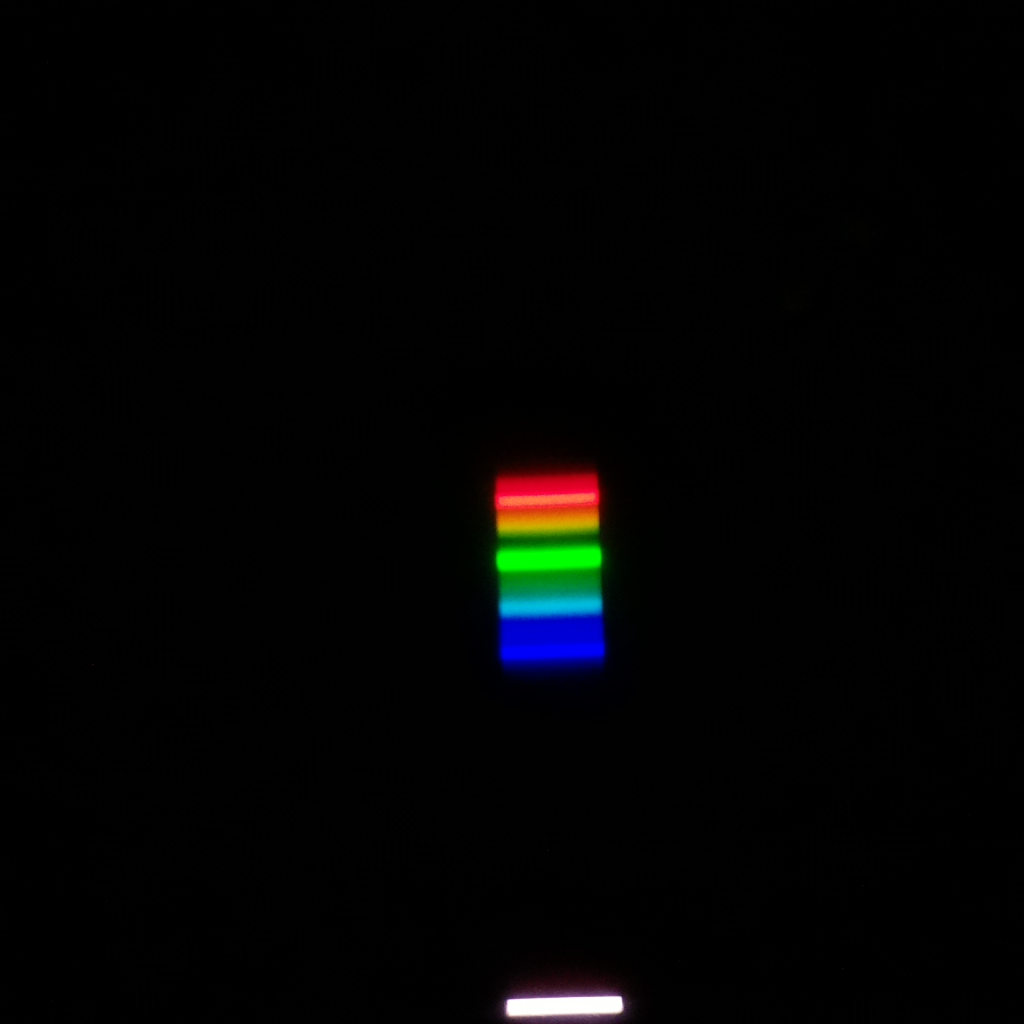
\includegraphics[scale=0.15]{calibrovka.jpg}}
                \caption{Cпектр ртутной лампы, отражённый от белого листа бумаги}
\end{figure}

\begin{figure}[h]
			\center{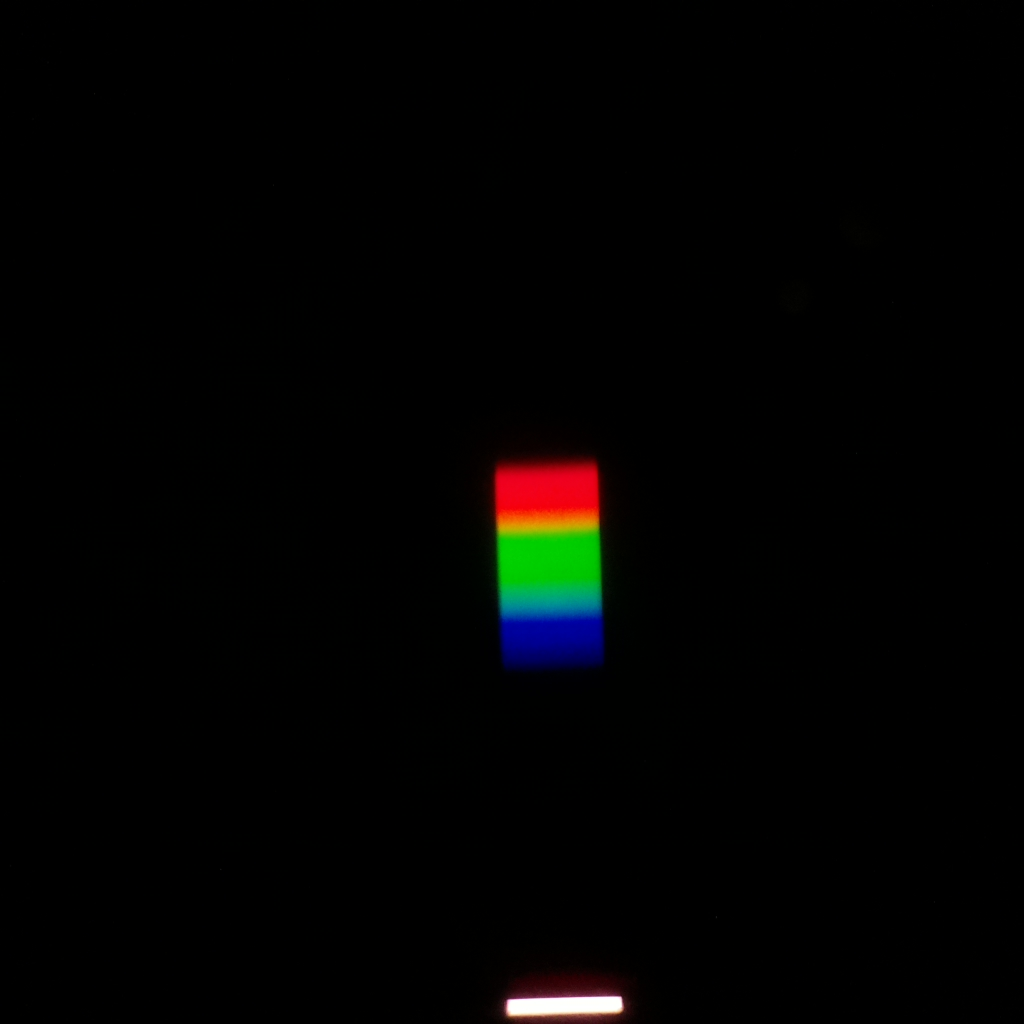
\includegraphics[scale=0.15]{white.jpg}}
                \caption{Cпектр лампы накаливания, отражённой от белого листа бумаги}
\end{figure}

\begin{figure}[h]
			\center{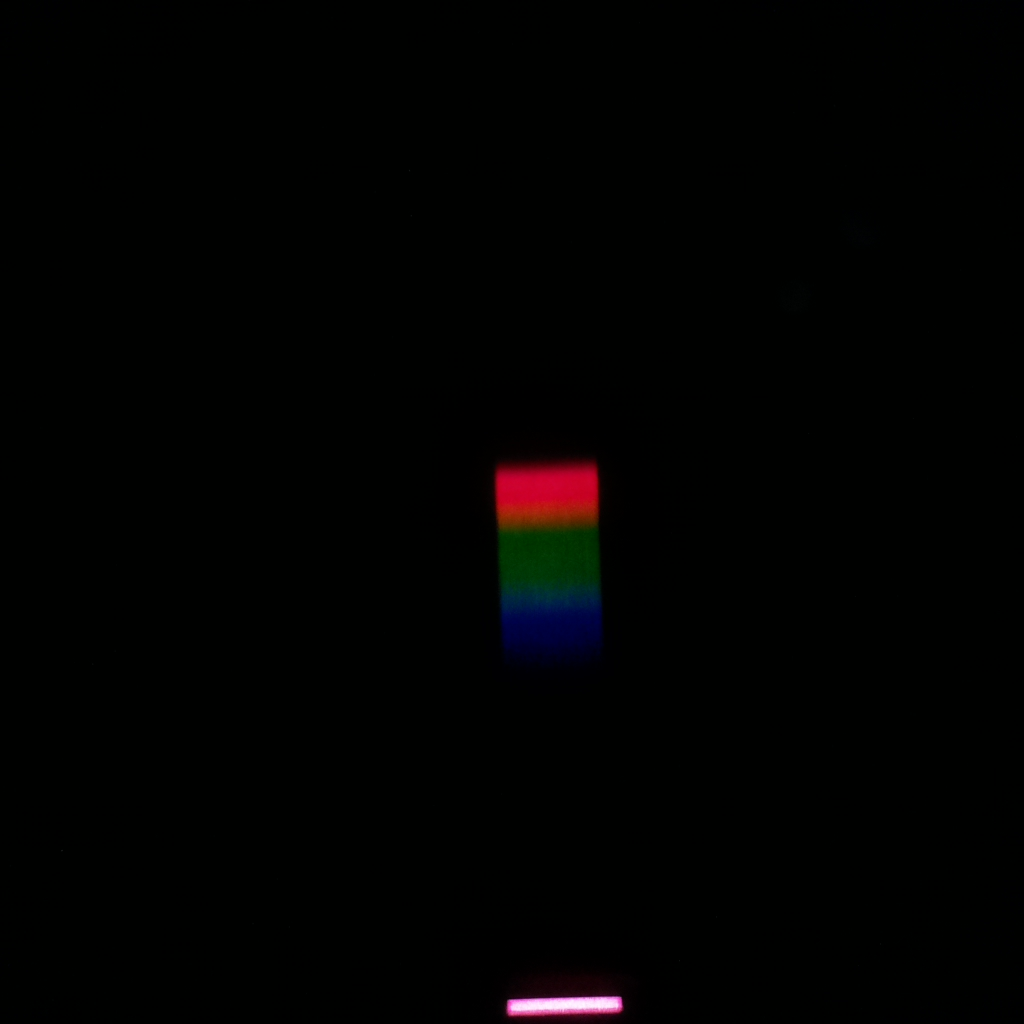
\includegraphics[scale=0.15]{red.jpg}}
                \caption{Спектр лампы накаливания, отражённый от красного листа бумаги}
\end{figure}

\begin{figure}[h]
			\center{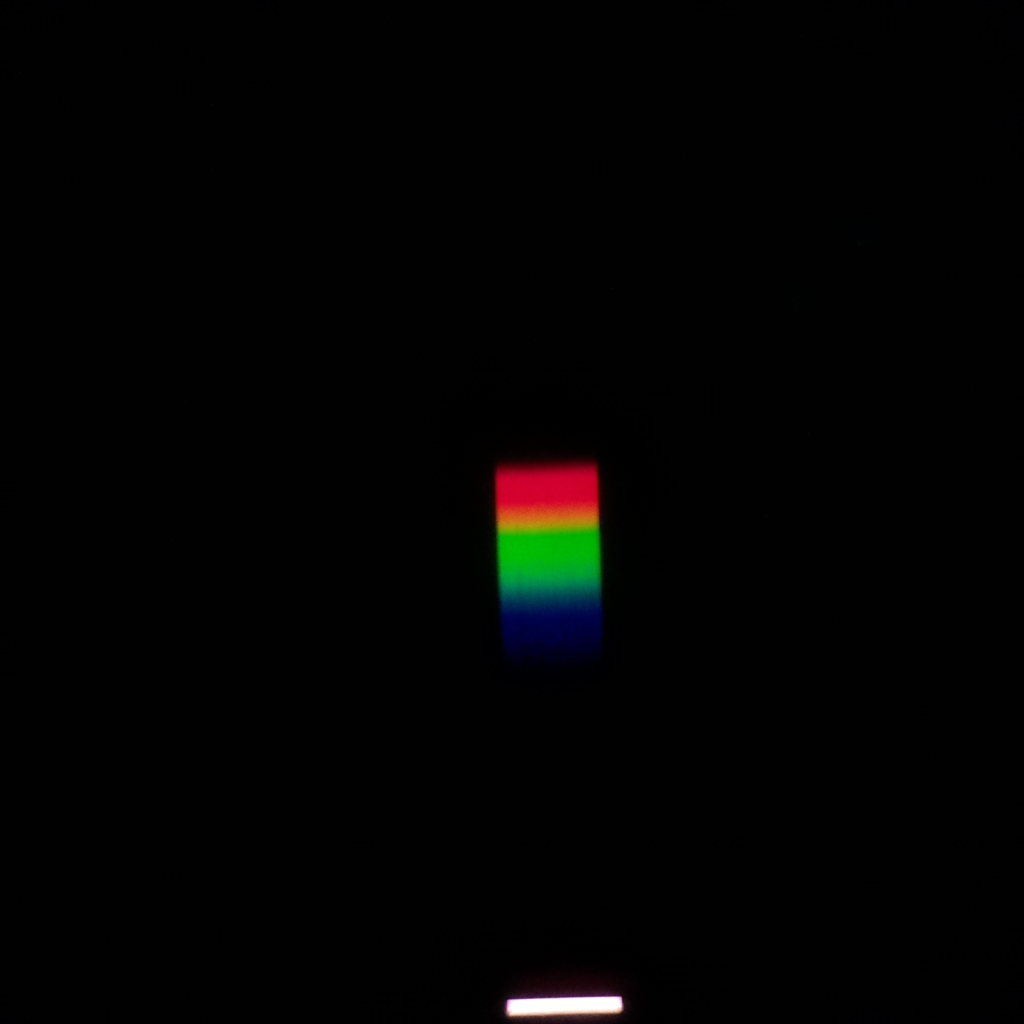
\includegraphics[scale=0.15]{yellow.jpg}}
                \caption{Спектр лампы накаливания, отражённый от жёлтого листа бумаги}
\end{figure}

\begin{figure}[h]
			\center{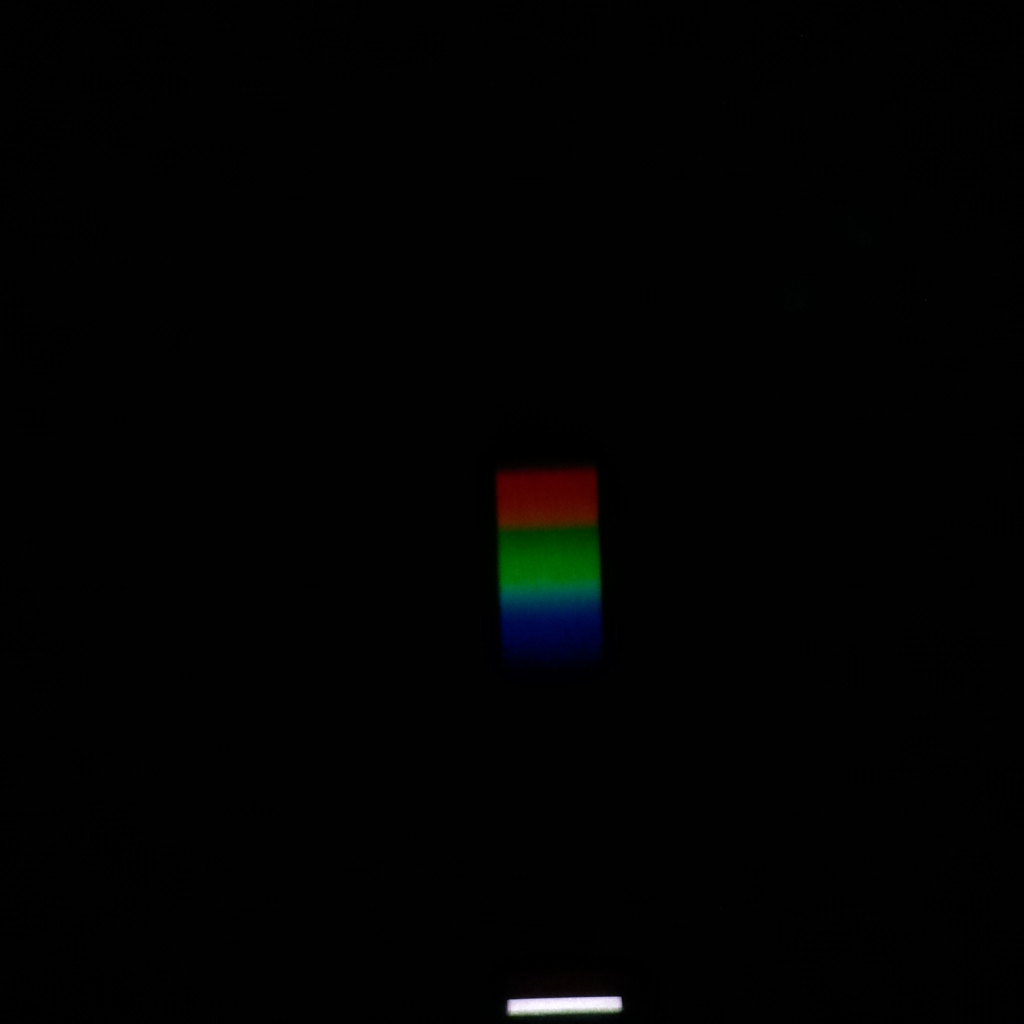
\includegraphics[scale=0.15]{green.jpg}}
                \caption{Спектр лампы накаливания, отражённый от зелёного листа бумаги}
\end{figure}

\begin{figure}[h]
			\center{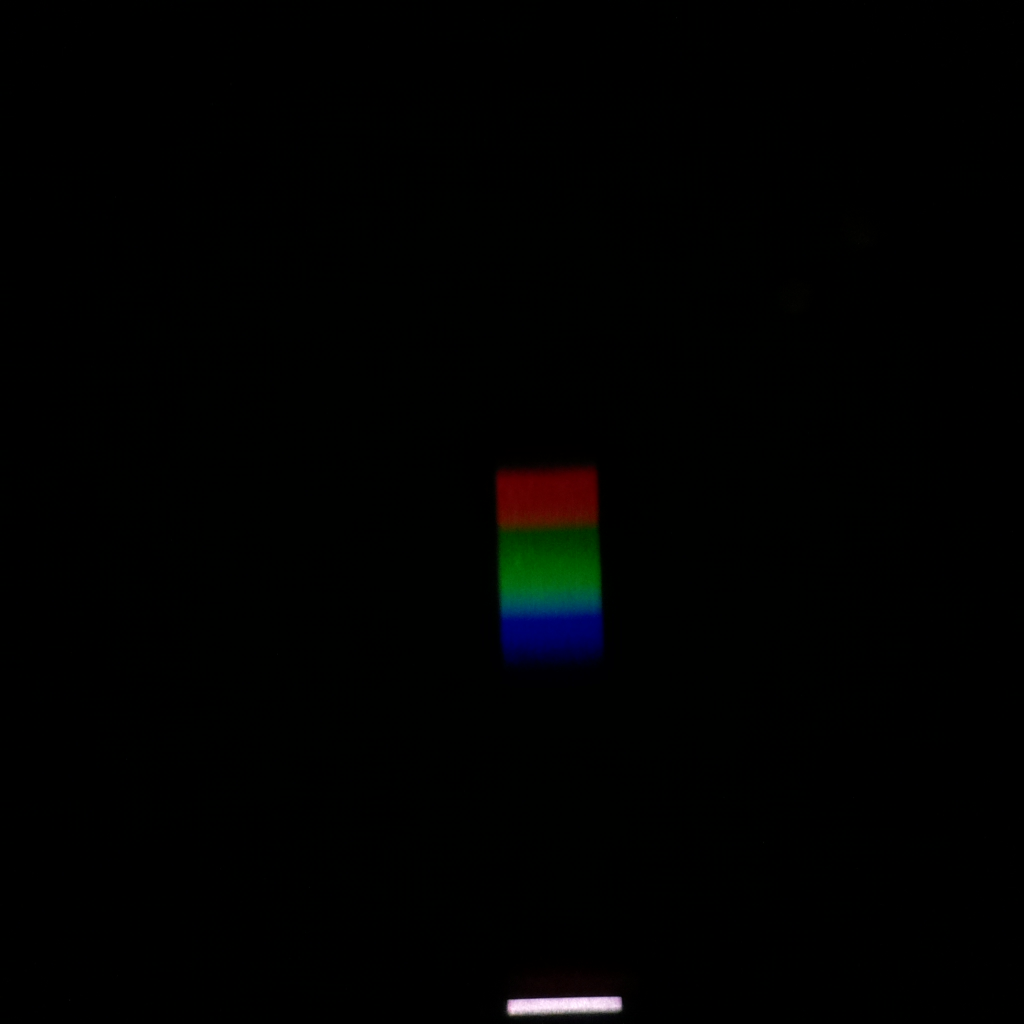
\includegraphics[scale=0.15]{blue.jpg}}
                \caption{Спектр лампы накаливания, отражённый от синего листа бумаги}
\end{figure}

\clearpage
\subsection{Программа эксперимента}


\begin{itemize}
\item получим фотографию спектра ртутной лампы, отраженного от белого листа бумаги
\item получим фотографии спектров лампы накаливания, отраженных от листов бумаги разных цветов
\item сохраним данные на git hub
\end{itemize}


\section{Обработка данных}
\subsection{Методика обработки изображения}

\begin{itemize}
\item с помощью imageio преобразовали изображение в трехмерный массив, где третье измерение это цвет через RGB
\item обрезка изображения
\end{itemize}


\subsection{Методика обработки данных}
\begin{itemize}
    \item используя библиотеки NumPy и Matplotlib, построим графики зависимости интенсивности света от относительного номера пикселя
    \item с помощью калибровки преобразуем этот график в график зависимости интенсивности света от длины волны
    \item приняв альбедо белого листа бумаги за 1, построим график зависимости альбедо от длины волны


\end{itemize}
\section{Код программы}

\subsection{Скрипты получения и обработки изображений и функции}
\url{https://github.com/yakov7podkova/get-labs}
\section{Эксперимент}
\subsection{Калибровка}

\begin{figure}[h]
			\center{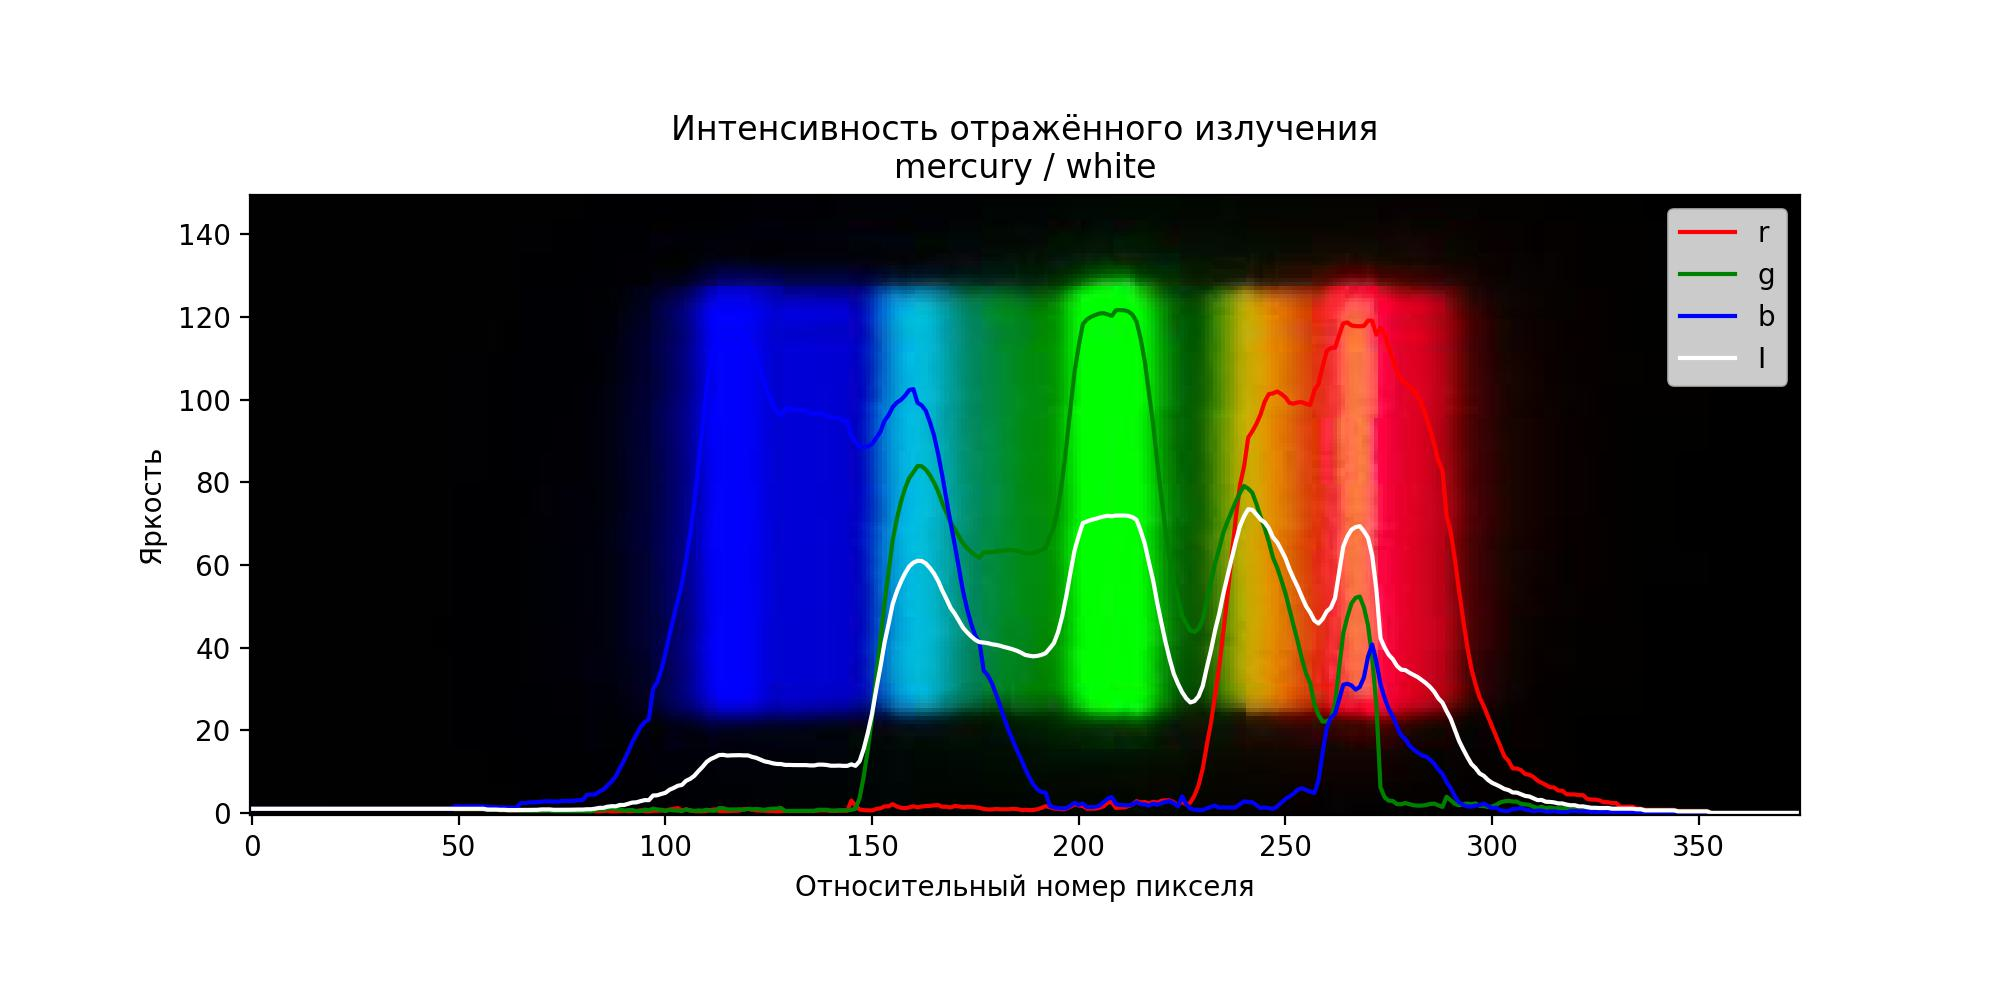
\includegraphics[scale=0.5]{calibrovka_plot.jpg}}
\end{figure}

\clearpage
\subsection{Графики интенсивностей}

\begin{figure}[h]
			\center{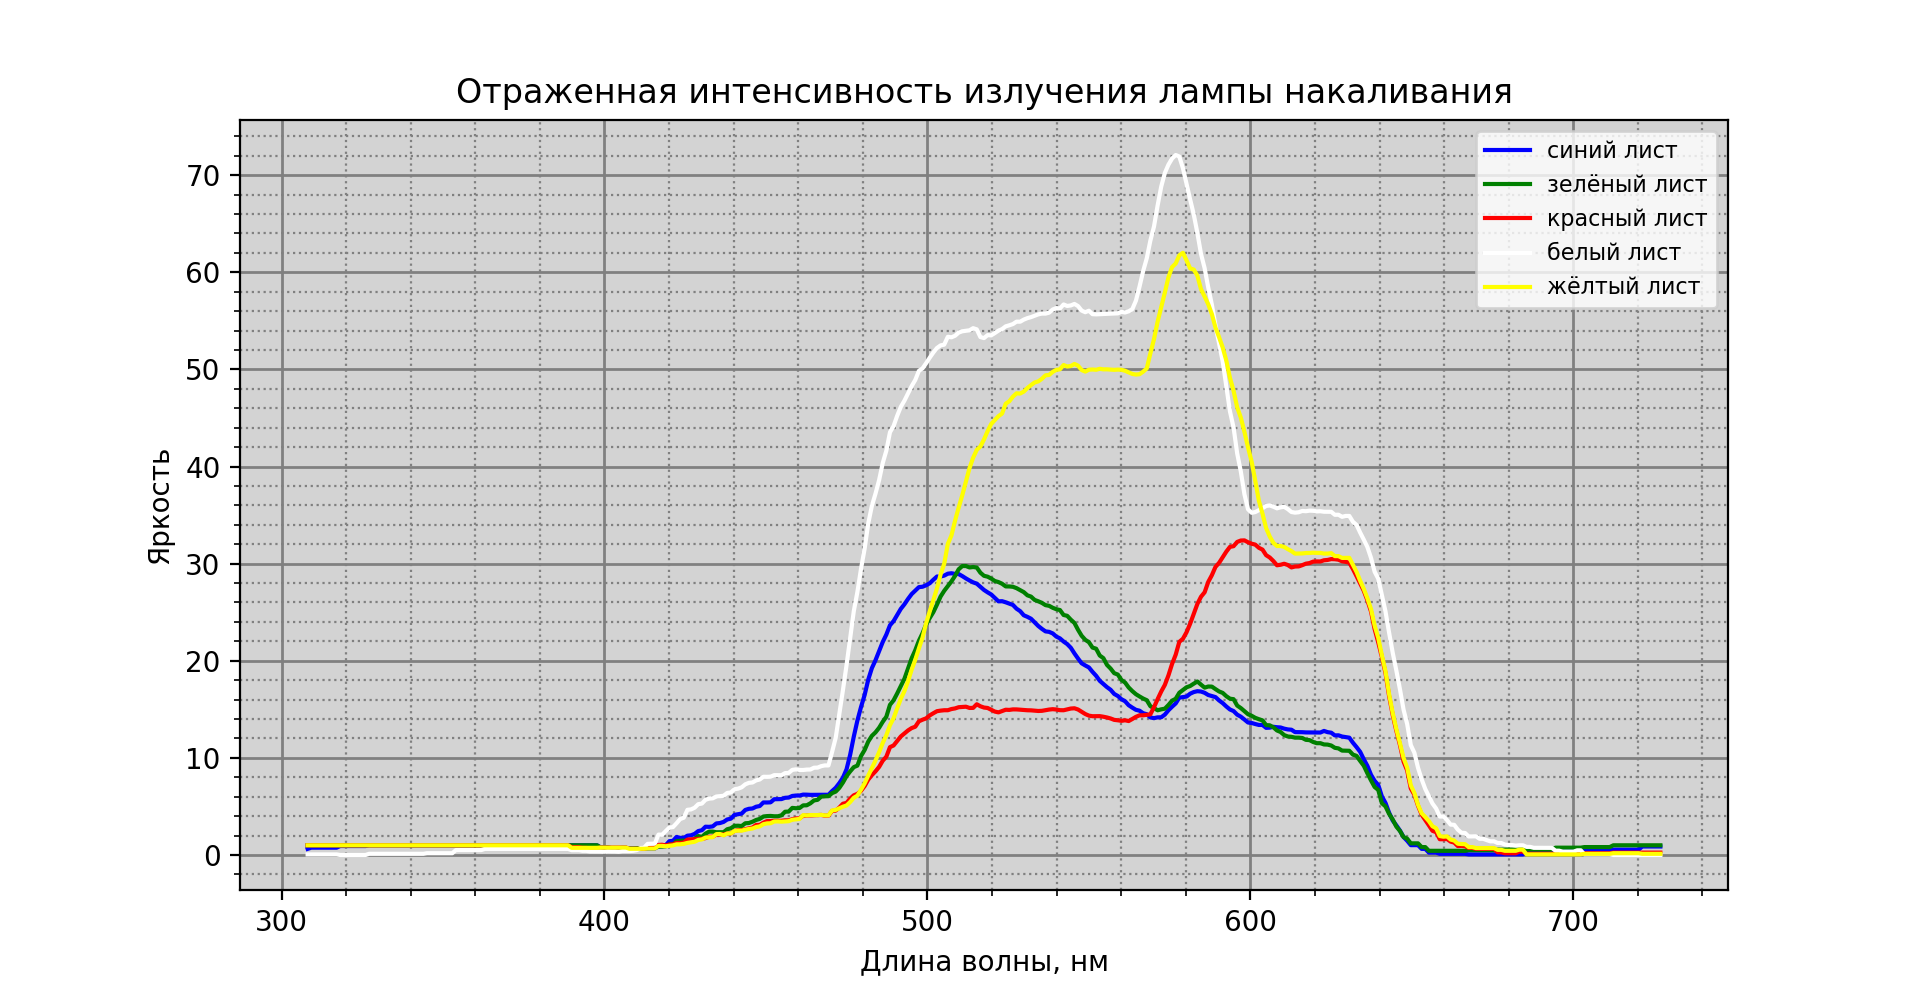
\includegraphics[scale=0.7]{intensites.png}}
\end{figure}

\subsection{График альбедо}

\begin{figure}[h]
			\center{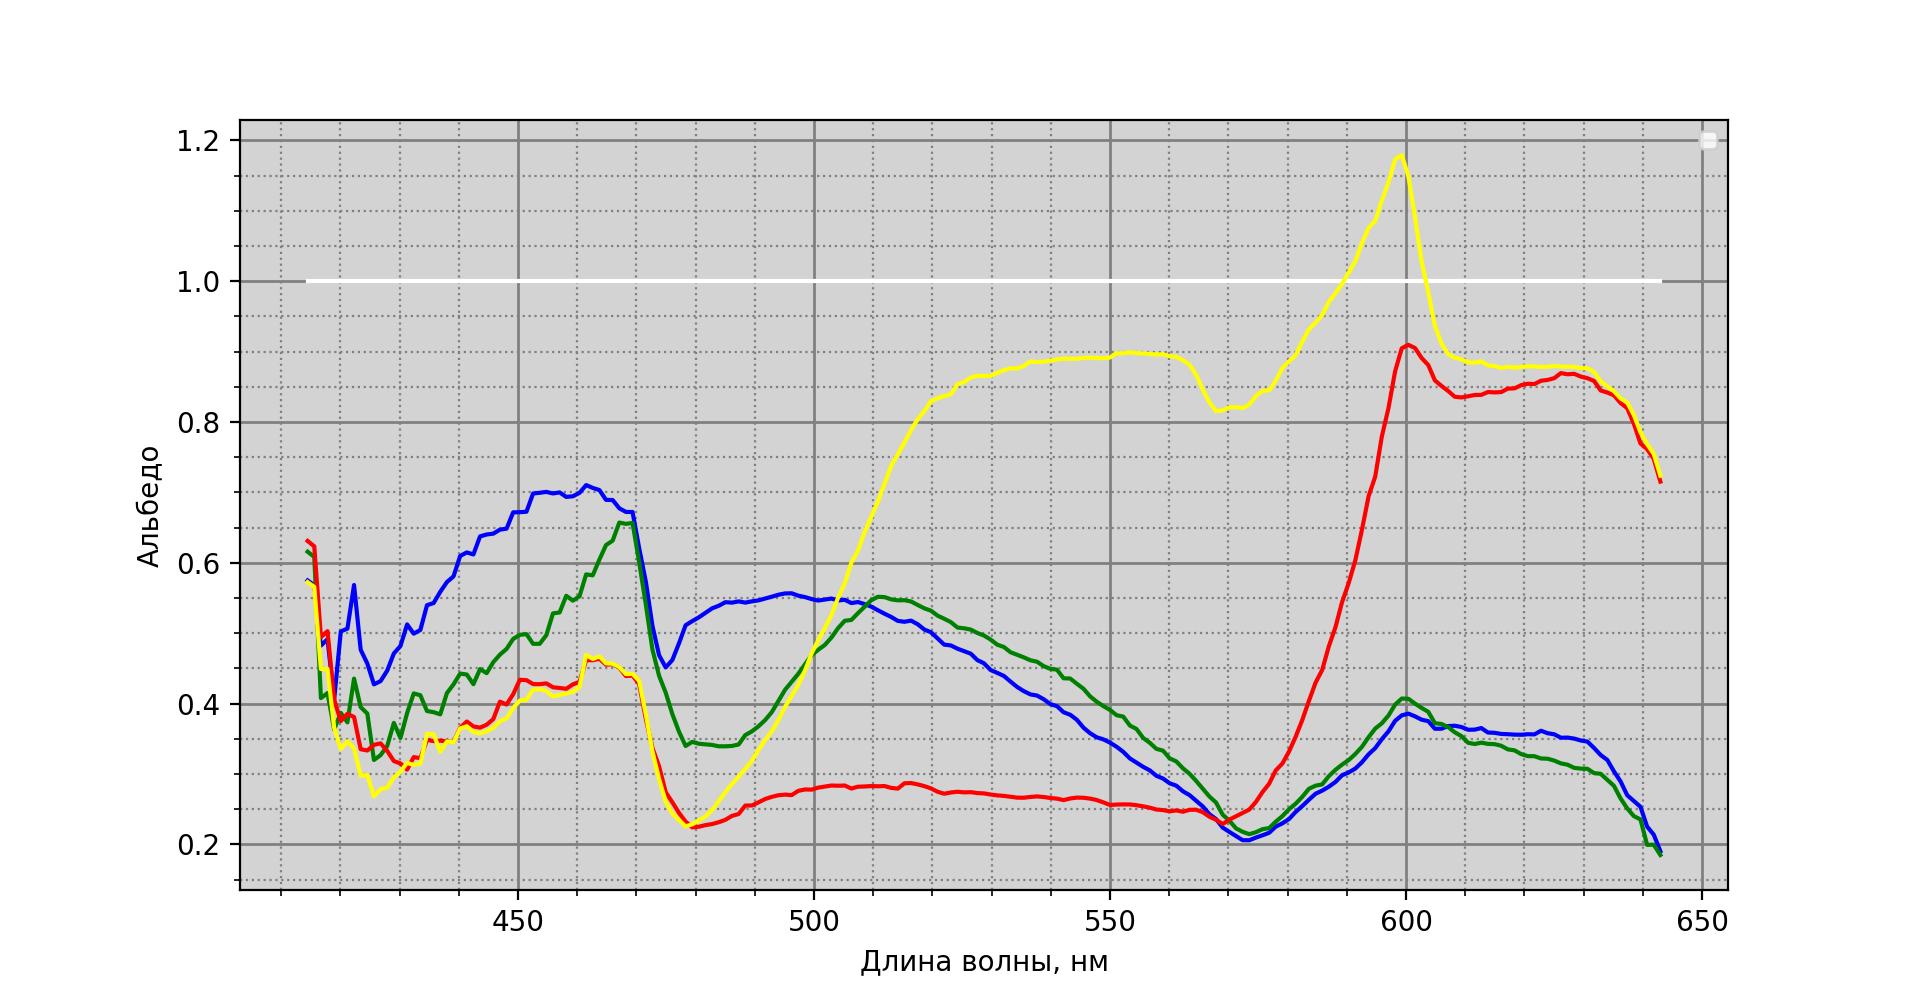
\includegraphics[scale=0.6]{albedo.png}}
   
\end{figure}

\section{Результаты}
Наибольшую интенсивность отраженного света имеет белый цвет, на втором месте желтый.
\section{Итоги лабораторной работы}
В результате лабораторной работы мы изучили зависимость альбедо отражающей поверхности от её цвета в видимой области спектра. Научились работать с модулем picamera, написали скрипты для работы с матрицей и полученными изображениями.

 \end{document}